%%
%% Commands for TeXCount
%TC:macro \cite [option:text,text]
%TC:macro \citep [option:text,text]
%TC:macro \citet [option:text,text]
%TC:envir table 0 1
%TC:envir table* 0 1
%TC:envir tabular [ignore] word
%TC:envir displaymath 0 word
%TC:envir math 0 word
%TC:envir comment 0 0
%%
%% Graph-CPO — submission to The Web Conference (WWW).
%% For anonymous review: \documentclass[sigconf, anonymous, review, screen]{acmart}
%% For camera ready:     \documentclass[sigconf]{acmart}  (+ real authors/rights)
%%
\documentclass[sigconf, anonymous, review, screen]{acmart}

\AtBeginDocument{%
  \hypersetup{
    colorlinks=true,
    citecolor=blue,
    linkcolor=blue,
    urlcolor=blue
  }%
  \providecommand\BibTeX{{%
    Bib\TeX}}}

    
%% Rights management: replace with the values from the rights confirmation
%% email at camera-ready time (see cross-check.txt, item B1).
% \setcopyright{acmlicensed}
% \copyrightyear{2027}
% \acmYear{2027}
% \acmDOI{XXXXXXX.XXXXXXX}
% \acmISBN{978-1-4503-XXXX-X/2027/06}
%% Conference details: confirm against the CFP/rights e-mail (cross-check.txt, B1).
\acmConference[WWW '27]{Proceedings of the ACM Web Conference 2027}{Date TBD}{Dublin, Ireland}

\usepackage{xcolor}
\usepackage{booktabs}
\usepackage{tabularx}
\usepackage{graphicx}
\usepackage{float}
%% Note: do NOT load amssymb here -- acmart loads newtxmath first, which
%% already defines \Bbbk/\checkmark/\mathbb, so amssymb would collide.
\usepackage{amsmath}

%% Tightened float spacing (page budget: 8 pages of main content).
\setlength{\textfloatsep}{10pt plus 2pt minus 2pt}
\setlength{\floatsep}{6pt plus 2pt minus 2pt}
\setlength{\intextsep}{8pt plus 2pt minus 2pt}
\setlength{\dbltextfloatsep}{10pt plus 2pt minus 2pt}
\setlength{\dblfloatsep}{6pt plus 2pt minus 2pt}
%% Kernel defaults: captions 10pt above, displays 12pt above/below.
\setlength{\abovecaptionskip}{3pt}
\setlength{\abovedisplayskip}{8pt plus 2pt minus 4pt}
\setlength{\abovedisplayshortskip}{4pt plus 2pt minus 4pt}
\setlength{\belowdisplayskip}{8pt plus 2pt minus 4pt}
\setlength{\belowdisplayshortskip}{4pt plus 2pt minus 4pt}

\newcommand{\ourmethod}{{Graph-CPO}}

% Professional light colors for highlighting
\definecolor{lightgreen}{HTML}{E8F5E8}     % Very light green background
\definecolor{lightred}{HTML}{FFF2F2}       % Very light red background
\definecolor{textgreen}{HTML}{2E7D32}      % Dark green text
\definecolor{textred}{HTML}{C62828}        % Dark red text

% Custom commands for superscripts with background highlighting
\newcommand{\improve}[1]{\textsuperscript{\colorbox{lightgreen}{\textcolor{textgreen}{\tiny +#1}}}}
\newcommand{\decline}[1]{\textsuperscript{\colorbox{lightred}{\textcolor{textred}{\tiny -#1}}}}


%%
%% end of the preamble, start of the body of the document source.
\begin{document}

\title{Graph-CPO: Graph-Grounded Contrastive Pedagogical Optimization for Socratic Question Generation}

%% Authors: add real names/affiliations at camera-ready (non-anonymous) stage.
%% The `anonymous' option masks this block during review.
\author{Anonymous Author(s)}
\email{anon@example.org}
\affiliation{%
  \institution{Anonymized for review}
}
\renewcommand{\shortauthors}{Anonymous Author(s)}

\begin{abstract}

Math word problems (MWPs) benefit from pedagogical scaffolding through Socratic questioning, yet automating effective question sequences remains challenging. Existing approaches treat question generation as static text-to-text tasks, ignoring the temporal dependencies among mathematical operations and intermediate reasoning steps. We address this by formalizing Socratic questioning as a finite-horizon sequential decision process, where each sub-question targets a specific reasoning dependency.
We propose \textit{\textbf{Graph-CPO} (\textbf{G}raph-grounded \textbf{C}ontrastive \textbf{P}edagogical \textbf{O}p\-timization)}, a reinforcement learning framework that conditions question generation on a Semantic Dependency Graph constructed from the problem structure. By employing dynamic reward weighting with independently normalized dimensions, Graph-CPO prevents signal domination by trivial objectives while guiding the policy toward logically coherent question sequences.
Extensive evaluation demonstrates that Graph-CPO generates superior sub-questions that significantly improve automated solver accuracy (+8.52 points average improvement over the same backbone) and achieves a 95.6\% sequence validity rate, competitive with systems using models $20\times$ larger. Human evaluation confirms higher coherence and pedagogical alignment compared to baselines.

\end{abstract}

\begin{CCSXML}
<ccs2012>
   <concept>
       <concept_id>10010147.10010178.10010179.10010182</concept_id>
       <concept_desc>Computing methodologies~Natural language generation</concept_desc>
       <concept_significance>500</concept_significance>
       </concept>
   <concept>
       <concept_id>10010147.10010257.10010258.10010261</concept_id>
       <concept_desc>Computing methodologies~Reinforcement learning</concept_desc>
       <concept_significance>500</concept_significance>
       </concept>
   <concept>
       <concept_id>10010405.10010489</concept_id>
       <concept_desc>Applied computing~Education</concept_desc>
       <concept_significance>300</concept_significance>
       </concept>
 </ccs2012>
\end{CCSXML}

\ccsdesc[500]{Computing methodologies~Natural language generation}
\ccsdesc[500]{Computing methodologies~Reinforcement learning}
\ccsdesc[300]{Applied computing~Education}

\keywords{Graph-CPO, Semantic Dependency Graph, Socratic Question Generation, Reinforcement Learning for Education, Math Word Problem Solving.}

\maketitle


\section{Introduction}

Socratic questioning guides problem solving through a sequence of purposeful inquiries \cite{kestin2025ai}.
For math word problems (MWPs), automating this process is difficult because useful questions must be fluent, mathematically valid, and aligned with the problem's latent reasoning structure. Prior work suggests that well-designed question sequences can improve both human and automated reasoning \cite{ang2023socratic}. However, most question generation (QG) methods treat generation as a static text-to-text task, which often ignores the temporal dependencies among quantities, operations, and intermediate variables \cite{scaria2024automated, li2024planning}. Consequently, generated questions may be redundant, weakly ordered, or disconnected from the final solution.

We argue that effective Socratic sub-question generation for MWPs requires two properties: \textbf{targetedness}, where each question addresses the most informative unresolved reasoning step, and \textbf{purpose-orientation}, where the sequence progressively advances the solver toward the final answer. To capture these properties, we formulate Socratic sub-question generation as a finite-horizon sequential decision process. At each timestep, the policy observes the problem, previous questions, and a graph-based reasoning state, then selects the next question as an action that should resolve a specific dependency in the solution path.

\begin{figure}[htbp]
\centering
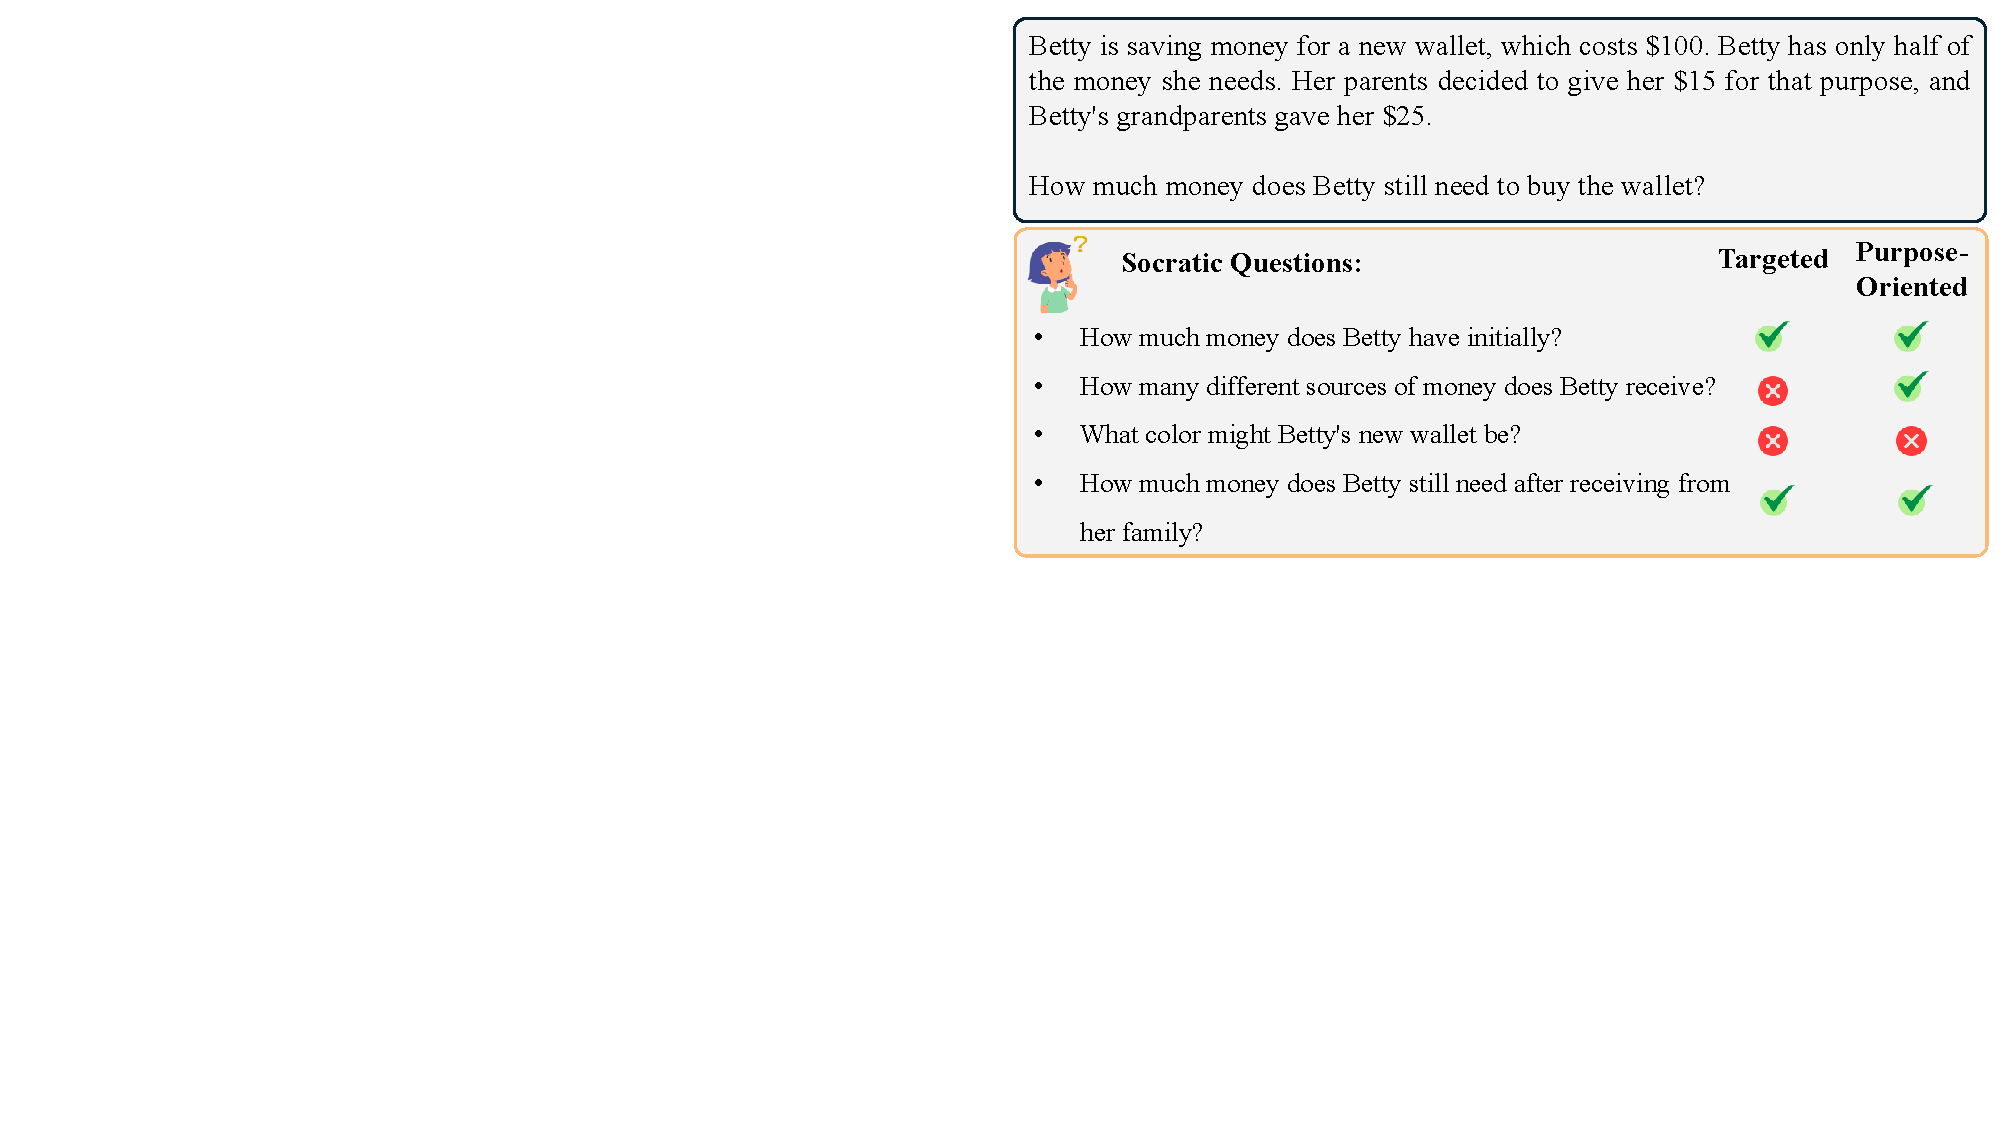
\includegraphics[width=0.90\linewidth]{01.Figures/Introduction.pdf}
\caption{Socratic questioning as a sequential decision process over an MWP: at each timestep the policy observes the problem, the previously asked sub-questions, and the current reasoning state, and targets the next unresolved reasoning dependency in the solution path.}
\label{fig:introduction}
\end{figure}

Optimizing such a policy is challenging because pedagogical quality depends on heterogeneous objectives, including relevance, logical coherence, and structural validity. Directly aggregating these rewards can cause \emph{reward collapse}: as training progresses, easy-to-optimize objectives such as format adherence saturate and dominate the aggregate learning signal, so that apparent progress in the scalarized reward masks stagnation or degradation of the harder reasoning-oriented rewards \cite{shao2024deepseekmath, liu2026gdpo}. To address this, we propose \textbf{Graph-CPO}, a graph-grounded reinforcement learning framework for Socratic question generation. Graph-CPO first constructs a Semantic Dependency Graph for each MWP, then maps frontier nodes in the graph to graph-conditioned question plans. During optimization, it uses a contrastive relevance reward to align questions with the current target node while penalizing repetition of resolved nodes. It further applies independently normalized reward dimensions and curriculum-based weighting to balance format, relevance, and coherence throughout training.

Our contributions are as follows:
\begin{enumerate}
    \item We formulate Socratic sub-question generation for MWPs as a finite-horizon sequential decision process grounded in a Semantic Dependency Graph, and propose Graph-CPO, a multi-objective reinforcement learning approach that combines graph-grounded contrastive rewards with independently normalized, curriculum-weighted reward dimensions to enable targeted and purpose-oriented Socratic questioning.

    \item We investigate the following research questions:
        \begin{itemize}
          \item \textbf{(RQ1):} \textit{Does incorporating Socratic sub-questions improve solution accuracy in math word problems?}
          \item \textbf{(RQ2):} \textit{Which structural and sequential properties are essential for effective Socratic questioning under a decision-theoretic framework?}
        \end{itemize}

    \item We provide a comprehensive empirical evaluation and ablation analysis showing that our framework generates question sequences with higher coherence and precise target alignment, which significantly improve both automated solver accuracy (+8.52 points on average) and subjective human quality ratings.

\end{enumerate}




\section{Related Work}
Socratic questioning is a cornerstone of educational pedagogy \cite{wood1976role}; in mathematics education it appears as funneling interactions that guide students toward key concepts \cite{wood1994patterns}. LLM-based systems now simulate Socratic dialogue to strengthen mathematical reasoning, from prompt-based tutors \cite{ding2024boosting, xi2025investigating, adewumi2026findings} to ideators that decompose problems into sequenced sub-questions \cite{lei2025motivgraph}, alongside studies of AI versus human tutors and of reviving Socratic methods in distance education \cite{fakour2025socratic, stamatellos2025socratic}.

Educational question generation (QG) with LLMs spans Bloom's-taxonomy assessment generation \cite{scaria2024automated, duong2024bloomllm}, multiple-choice generation \cite{biancini2024multiple}, controllable prompt patterns \cite{li2024planning}, and RLHF-driven multimodal systems \cite{mubarak2025quesgenie} (see also reviews of neural QG in education \cite{al2024review}). Reinforcement learning further shapes QG through graph-to-sequence and answer-driven generation \cite{guan2023reinforcement, chen2019reinforcement, wang2020answer}, fine-tuning of LLMs for educational question generation \cite{lamsiyah2024fine}, and multi-agent frameworks for math problem generation \cite{fahad2023reinforcement}.

Math word problem (MWP) solving with LLMs has advanced through estimation verification and symbolic solvers \cite{piehl2025solving}, abstract-reasoning probes without explicit numbers \cite{cheng2025can}, template-driven paraphrasing \cite{kang2025template}, iterative distractor refinement \cite{yang2025iterative}, step-by-step correction \cite{li2025step}, and multimodal benchmarks \cite{zhang2024mathverse}, with human-cognition perspectives surveyed in \cite{huang2025foundation}. Group-sampling RL objectives \cite{shao2024deepseekmath} achieve high scores on MATH and GSM8K, but they optimize single-reward trajectories---precisely the setting that lacks the robustness needed for the multi-objective optimization behind pedagogical scaffolding.

Beyond task-specific reward design, aggregating heterogeneous rewards into a single scalar is a long-standing challenge in RL: naive scalarization lets easy-to-saturate or high-variance dimensions dominate the learning signal \cite{skalse2022defining, gao2023scaling}. Existing remedies include stabilizing value functions across reward scales (PopArt \cite{hessel2021popart}) and normalizing each reward dimension separately inside policy-gradient updates \cite{liu2026gdpo}. In language-model alignment, \emph{reward hacking} has been extensively documented \cite{gao2023scaling, skalse2022defining}: the agent maximizes a proxy objective while degrading the true objective. GRPO-style objectives \cite{shao2024deepseekmath} normalize rewards within a sampled group, but typically scalarize multiple dimensions \emph{before} normalization---the exact setting in which easy objectives mask harder ones. Graph-CPO instead normalizes each pedagogical dimension independently and only then combines them under a curriculum; we show empirically that this prevents format adherence from masking relevance and coherence during training (Appendix Figure~\ref{fig:training_comparison}).

Our work redefines Socratic questioning as a finite-horizon trajectory over an explicit reasoning structure and contributes a multi-objective optimization scheme for navigating it: a graph-grounded contrastive reward makes each question \textbf{targeted}, while independently normalized, curriculum-weighted reward dimensions keep the training signal balanced so that the sequence remains \textbf{purpose-oriented}, preventing easy objectives from dominating optimization.



\begin{figure*}[!ht]
    \centering
  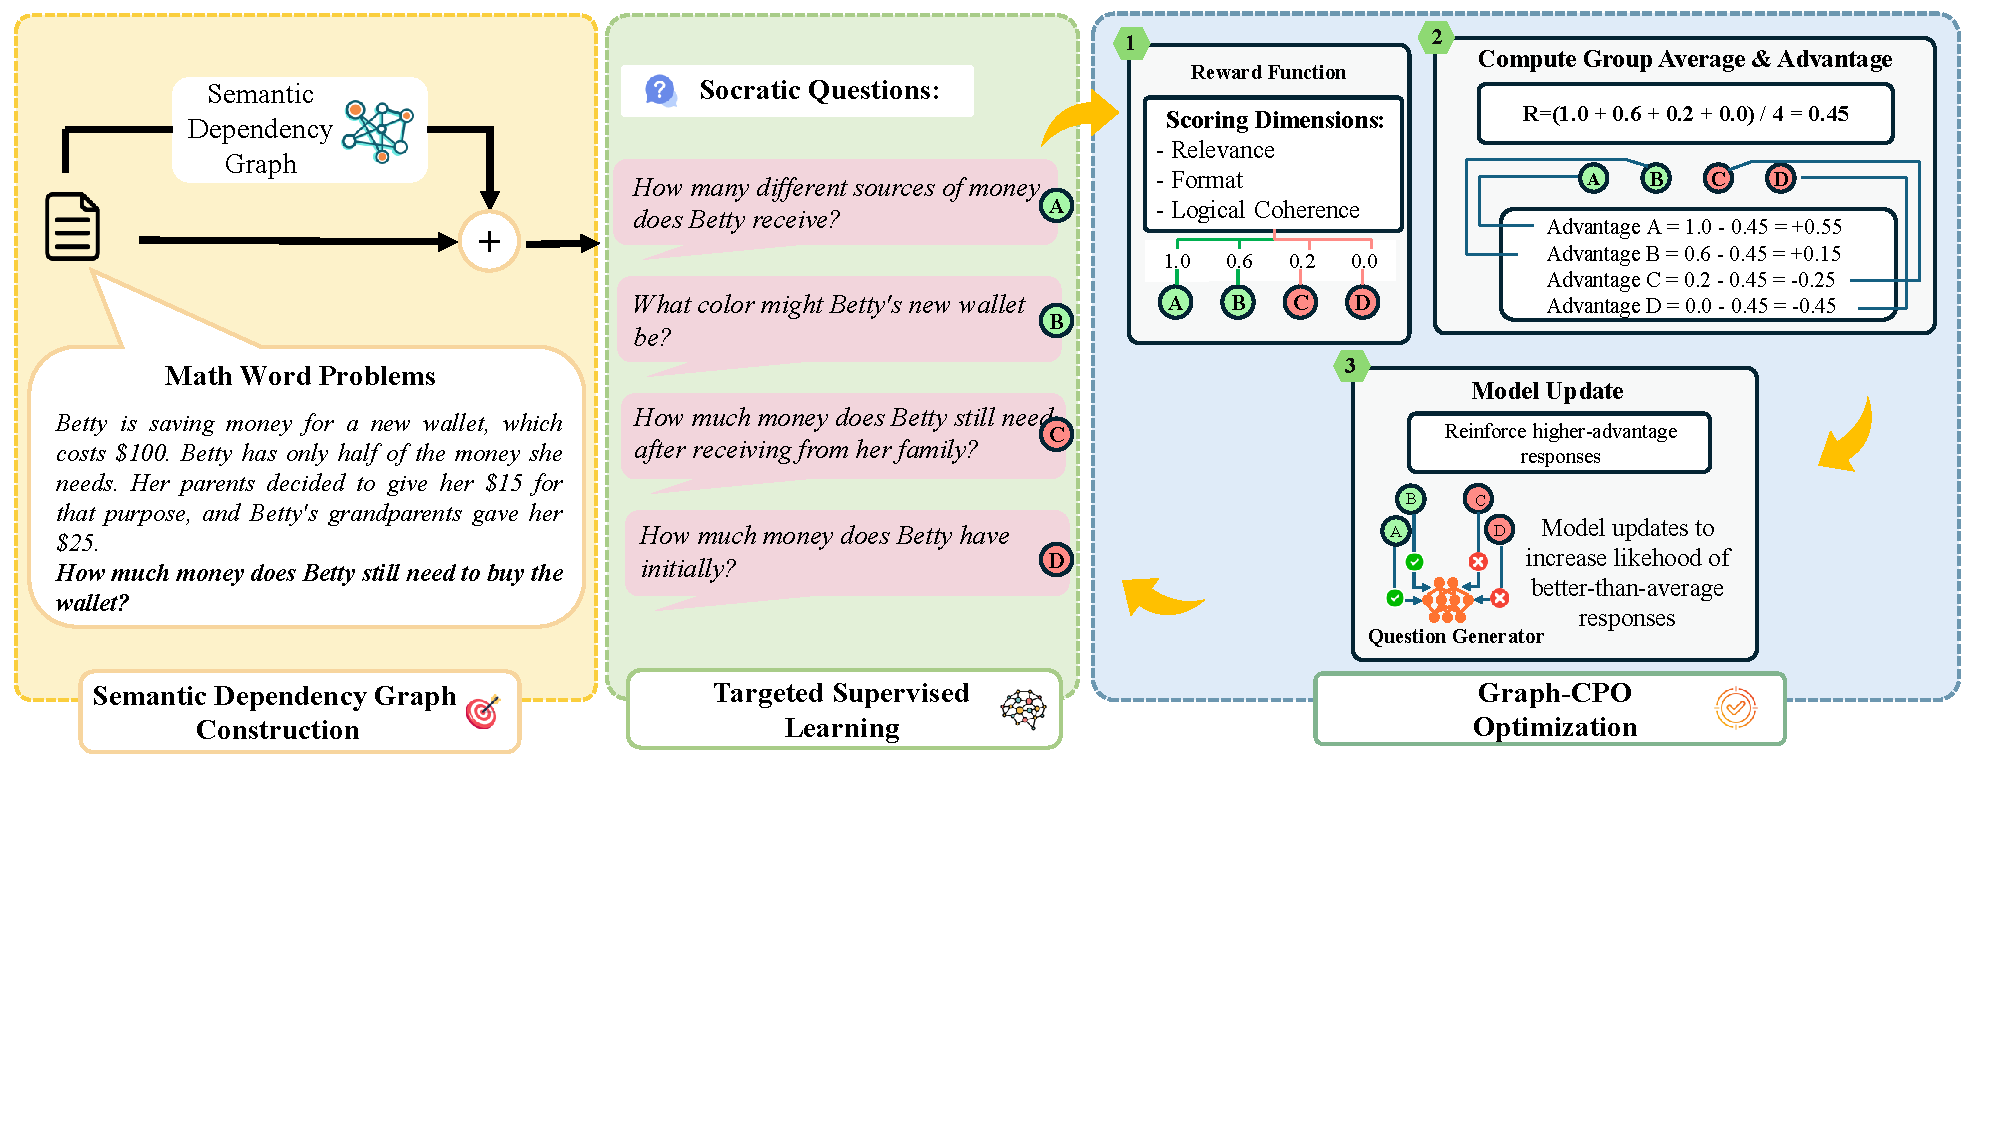
\includegraphics[width=0.80\textwidth]{01.Figures/Overall_Figure_v1.pdf}
  \caption{Overall processing pipeline of the proposed framework integrating Graph-CPO. It utilizes the Semantic Dependency Graph to identify the reasoning frontier for targeted question generation. Then, a warm-start strategy is set for reinforcement learning via targeted supervised learning. Subsequently, Graph-CPO optimizes sub-question generation via adaptive reward modeling and curriculum-based learning.}

  \label{fig:teaser}
\end{figure*}



\section{Methodology}

In this section, we describe Graph-CPO as a structured, three-phase pipeline where each phase produces essential components that the subsequent phase requires. Figure~\ref{fig:teaser} depicts our overall approach. Particularly, \textbf{Phase 1 - Semantic Dependency Graph Construction and Question Planning} (Sections~\ref{sec:graph} and~\ref{sec:g2q}): we construct a Semantic Dependency Graph ($\mathcal{G}$) that transforms unstructured problem text into an explicit topological representation of reasoning dependencies, and convert the current graph state into a compact, graph-conditioned question plan. The graph serves as the structural foundation that provides the state representation required for all subsequent components.
\textbf{Phase 2 - Targeted Supervised Learning} (Section~\ref{sec:init}): building directly on the structured graph from Phase 1, we train a Graph-Augmented Policy that conditions question generation on specific nodes in $\mathcal{G}$. This step produces a warm-started policy $\pi_\theta$ that mitigates cold-start instabilities in reinforcement learning while ensuring graph-aware question generation.
\textbf{Phase 3 - Graph-CPO Optimization} (Section~\ref{sec:cpo}): we integrate the graph structure and the initialized policy through the core Graph-CPO algorithm, which optimizes the question generator by decoupling reward dimensions and applying dynamic weighting strategies. By anchoring the multi-objective optimization to the topological roadmap from Phase 1 and the stable initialization from Phase 2, Graph-CPO effectively bridges local reasoning steps with global problem-solving objectives while preventing reward collapse.

\subsection{Semantic Dependency Graph for Targeted Sub-Question Generation}
\label{sec:graph}

Given an MWP $P$, we construct a directed acyclic \textbf{Semantic Dependency Graph}
$\mathcal{G}=(V,E,\tau,\rho,w)$, where each node $v\in V$ is a typed reasoning unit, each edge
$e=(u,v)\in E$ is a typed dependency, $\tau(\cdot)$ and $\rho(\cdot)$ denote node and edge types,
and $w_e\in[0,1]$ is the relation confidence. Unlike a generic syntactic parse, $\mathcal{G}$
represents a pedagogical solution topology: an edge $u\!\rightarrow\!v$ indicates that $u$ should be
identified or reasoned about before asking a question targeting $v$.

\begin{table}[t]
\centering
\scriptsize
\caption{Schema of the Semantic Dependency Graph.}
\label{tab:sdg_schema}

\begin{tabular}{p{0.18\columnwidth}p{0.4\columnwidth}p{0.23\columnwidth}}
\toprule
\textbf{Type} & \textbf{Definition} & \textbf{Example / Direction} \\
\midrule
\multicolumn{3}{l}{\textit{Node types}} \\
\textsc{Quantity} & Numerical value with unit or owner & ``12 apples'' \\
\textsc{Entity} & Person, object, group, or unit & ``Tom'', ``apples'' \\
\textsc{Variable} & Unknown or intermediate quantity & apples left \\
\textsc{Operation} & Arithmetic/reasoning operator & $+,-,\times,\div$, ratio \\
\textsc{Condition} & Constraint or comparison & ``twice'', ``after'' \\
\textsc{Goal} & Final asked quantity & ``how many remain?'' \\
\midrule
\multicolumn{3}{l}{\textit{Edge types}} \\
\textsc{quantity-of} & Quantity belongs to an entity & $q\!\rightarrow\!e$ \\
\textsc{op-input} & Node is input to an operation & $x\!\rightarrow\!op$ \\
\textsc{derive} & Operation produces a derived value & $op\!\rightarrow\!x$ \\
\textsc{condition} & Node participates in a constraint & $x\!\rightarrow\!c$ \\
\textsc{prerequisite} & Source must be resolved first & $u\!\rightarrow\!v$ \\
\textsc{goal-dep.} & Node is required for final goal & $u\!\rightarrow\!g$ \\
\bottomrule
\end{tabular}

\end{table}

\paragraph{Graph construction.}
The graph is built in three stages. First, a fine-tuned BERT sequence tagger extracts text spans and
assigns them to the node types in Table~\ref{tab:sdg_schema}. Explicit quantities are normalized with
their units, while operation and condition nodes are created from arithmetic cues such as
``left'', ``each'', ``twice'', or ``more than''. Second, candidate node pairs are formed when they occur
in the same sentence, share an entity/unit, are linked by an arithmetic cue, or connect to the final
goal. A biaffine relation classifier then predicts either one edge type in
Table~\ref{tab:sdg_schema} or \textsc{null}. Edges are oriented from prerequisite facts toward derived
variables and the goal. If the predicted graph contains a cycle, we remove the lowest-confidence edge
in the cycle until a valid Directed Acyclic Graph is obtained. The tagger and the biaffine classifier
are trained on silver labels distilled from the solution steps of 12{,}000 GSM8K/MathQA training
problems; the 1{,}000 expert-annotated graphs used for evaluation (Section~\ref{sec:sdg_eval}) are
held out and never used for training. Third, we encode $\mathcal{G}$ with a relation-aware GNN.
Each node is initialized by concatenating its span embedding, type embedding, and numeric features:

\[
\mathbf{h}^{(0)}_i = \operatorname{BERT}(v_i) \oplus \mathbf{e}_{\tau(v_i)} \oplus \phi_{\mathrm{num}}(v_i)
\]
The GNN updates node representations by relation type:

\[
\mathbf{h}^{(\ell+1)}_i =
\sigma\!\left(
W_0\mathbf{h}^{(\ell)}_i+
\sum_{r\in\mathcal{R}}\sum_{j\in\mathcal{N}_r(i)}
\frac{1}{c_{i,r}}W_r\mathbf{h}^{(\ell)}_j
\right),
\]
where $\mathcal{N}_r(i)$ denotes neighbors connected to $i$ by relation $r$. The final node embedding
$\mathbf{h}^{(L)}_i$ is used by the generator and by the graph-grounded relevance reward.

\paragraph{Frontier tracking and node resolution.}
At timestep $t$, the graph state is
$\mathcal{G}_t=(\mathcal{G},V^t_{\mathrm{res}},V^t_{\mathrm{unres}})$, where ``resolved'' means that
the corresponding reasoning dependency has already been covered by a generated sub-question. Initially,
$V^0_{\mathrm{res}}=\emptyset$ and $V^0_{\mathrm{unres}}=V$. The targetable reasoning frontier is

\begin{equation}
\mathcal{F}_t =
\{v\in V^t_{\mathrm{unres}}\cap V_Q
\mid \operatorname{Pre}(v)\subseteq V^t_{\mathrm{res}}\},
\label{eq:frontier}
\end{equation}
where $V_Q$ excludes purely entity nodes and $\operatorname{Pre}(v)$ denotes the prerequisite nodes of
$v$. Among frontier nodes, the next target $v_t$ is selected by the scoring rule of
Section~\ref{sec:g2q}, which prioritizes nodes closer to the goal, with larger prerequisite depth and
higher relation confidence.

After generation, $v_t$ is marked as resolved only if the question is both semantically aligned with
the target node and logically addresses its dependency:

\[
s_{\mathrm{sim}}=\cos(\operatorname{Enc}(q_t),\mathbf{h}^{(L)}_{v_t})\ge \tau_{\mathrm{sim}},
\]

\[
s_{\mathrm{nli}}=
P_{\mathrm{NLI}}(\mathrm{entail}\mid [P;\hat d(q_t)],d(v_t))
\ge \tau_{\mathrm{nli}},
\]
where $\hat d(q_t)$ is the declarative target extracted from the generated question and $d(v_t)$ is the verbalized target dependency. If either test fails, the node remains unresolved and the question receives a lower relevance/coherence reward during Graph-CPO optimization. This frontier-based update ensures that generated questions follow the graph topology rather than repeatedly querying already covered or downstream reasoning steps. Having established how we construct the Semantic Dependency Graph that encodes mathematical reasoning structure, we now describe how this graph guides the generation of targeted Socratic questions through a graph-to-question planning mechanism.



\subsection{Graph-to-Question Planning}
\label{sec:g2q}

The Semantic Dependency Graph is not passed to the generator as an unstructured object. Instead, at each timestep we convert the current graph state $\mathcal{G}_t$ (Section~\ref{sec:graph}) into a compact \textbf{Pedagogical Action Frame} that specifies exactly which reasoning dependency the next Socratic question should address.

\paragraph{Frontier node selection.}
Among the frontier nodes $\mathcal{F}_t$ of Equation~\eqref{eq:frontier}, we select the next target by:

\begin{equation}
\begin{split}
v_t = \arg\max_{v\in\mathcal{F}_t} \left[
\lambda_g \frac{1}{1+\operatorname{dist}(v,g)}
+ \lambda_d \operatorname{depth}(v) \right. \\
\left. + \lambda_c \bar{w}(v)
- \lambda_r \operatorname{red}(v) \right],
\end{split}
\label{eq:node_selection}
\end{equation}

where $g$ is the goal node, $\bar{w}(v)$ is the average confidence of edges incident to $v$, and
$\operatorname{red}(v)=\max_{u\in V^t_{\mathrm{res}}}\cos(\mathbf{h}^{(L)}_v,\mathbf{h}^{(L)}_u)$
penalizes revisiting already resolved reasoning units. If $V^t_{\mathrm{res}}=\emptyset$, the redundancy term is set to zero.

\paragraph{Pedagogical action frame.}
The selected node $v_t$ is converted into an action frame:
\begin{equation}
z_t =
\big(
d(v_t),\tau(v_t),\iota(v_t),
d(\operatorname{Pre}(v_t)),
d(\mathcal{N}_1(v_t)),
d(V^t_{\mathrm{res}})
\big),
\label{eq:action_frame}
\end{equation}
where $d(\cdot)$ verbalizes node spans, units, and edge labels; $\tau(v_t)$ is the node type; $\mathcal{N}_1(v_t)$ is the one-hop neighborhood; and $\iota(v_t)$ is the pedagogical intent derived from the node type, e.g., \textsc{identify-quantity}, \textsc{interpret-condition}, \textsc{select-operation}, or \textsc{derive-value}. The frame is serialized as a short control prompt:
\begin{quote}
\scriptsize
\textbf{Target:} $d(v_t)$;
\textbf{Intent:} $\iota(v_t)$;
\textbf{Prerequisites:} $d(\operatorname{Pre}(v_t))$;
\textbf{Local relation:} $d(\mathcal{N}_1(v_t))$;
\textbf{Avoid:} $d(V^t_{\mathrm{res}})$.
Ask exactly one Socratic question that helps derive the target without directly revealing the answer.
\end{quote}

\paragraph{Generator input.}
For Qwen3-32B, the actual generation input is:
\begin{equation}
x_t =
[P;\; q_{1:t-1};\; \operatorname{Ser}(z_t);\; \texttt{<question>}],
\end{equation}
where $P$ is the MWP text, $q_{1:t-1}$ are previous sub-questions, and $\operatorname{Ser}(z_t)$ is the serialized action frame. To incorporate continuous graph information, we additionally project the target-node and neighborhood embeddings into a graph prefix:

\begin{equation}
\mathbf{p}_t = W_p \left[\mathbf{h}^{(L)}_{v_t} \oplus \operatorname{Pool}_{u \in \mathcal{N}_1(v_t)} \mathbf{h}^{(L)}_u\right]
\end{equation}
The policy then samples:
\begin{equation}
q_t \sim \pi_\theta(\cdot \mid x_t,\mathbf{p}_t).
\end{equation}

Thus, the generator receives both a textual plan that is readable by the LLM and a graph embedding that preserves structural information from the GNN.

\paragraph{Binding questions to graph targets.}
Each generated question is explicitly associated with its target node $v_t$. Resolved nodes are included in the \textit{Avoid} field and are also penalized by the contrastive relevance reward, preventing the model from repeatedly asking about already covered dependencies. After generation, $v_t$ is marked as resolved only when the question passes the semantic-similarity and NLI checks of Section~\ref{sec:graph}; otherwise the graph state is unchanged and the question receives a lower reward during Graph-CPO optimization. This mechanism ensures that question generation follows the dependency topology of $\mathcal{G}$ rather than relying on unconstrained prompting.


\subsection{Warm-start Policy Initialization with Targeted Supervised Learning}
\label{sec:init}


To provide a stable starting point for the Graph-CPO optimization phase, we first initialize the policy $\pi_\theta$ via targeted supervised learning. This warm-start stabilizes subsequent reinforcement learning by constraining early policy updates to the manifold of syntactically valid and semantically meaningful questions, thereby reducing gradient variance and preventing policy collapse under sparse, long-horizon reward signals \cite{cobbe2021training}. We employ a Graph-Augmented Policy, which enhances a standard transformer encoder-decoder by fusing the problem text embeddings with structure-aware graph representations. This allows the decoder to attend not just to previous tokens, but to the topological state of the reasoning frontier. During this supervised warm-start phase, the policy is trained to imitate ground-truth Socratic sub-question sequences using a standard negative log-likelihood objective. These teacher sequences are constructed from the annotated solution steps of 8{,}000 training MWPs (4{,}000 GSM8K and 4{,}000 MathQA): each solution step is verbalized as one Socratic sub-question aligned to the corresponding graph node, yielding one teacher trajectory per problem. The loss function for this training is defined as:
\begin{equation}
    \mathcal{L}_{QG} = -\sum_{i=1}^{n} \log P_{\text{Dec}}(q_i \mid q_{1:i-1}; \operatorname{Enc}(P)),
    \label{eq:lqg}
\end{equation}
where $P_{\text{Dec}}(\cdot)$ denotes the decoder-defined conditional probability of generating the next sub-question under the current policy, parameterized by the transformer decoder. This autoregressive decoding ensures that the questions build upon each other logically, mirroring the sequential nature of mathematical reasoning.

\subsection{Graph-CPO: Graph-Grounded Contrastive Pedagogical Optimization}
\label{sec:cpo}

Supervised warm-starting makes the generator fluent, but it does not directly optimize long-horizon pedagogical utility. We therefore introduce \textbf{Graph-CPO}, a GRPO-style policy optimization method \cite{shao2024deepseekmath} that differs from scalar GRPO in two ways: rewards are first normalized independently by pedagogical dimension, and then combined through a curriculum-based weighting schedule. This prevents easy objectives, such as format adherence, from dominating harder graph-grounded reasoning signals.

\paragraph{Graph-conditioned supervised anchor.}
Given the action frame $z_t$ and graph prefix $\mathbf{p}_t$ from Section~\ref{sec:g2q}, we retain a supervised anchoring loss:
\begin{equation}
\mathcal{L}_{target}
=
-\sum_{t=1}^{H}
\log \pi_\theta
\left(
q_t^*
\mid
P,q_{<t}^*,\operatorname{Ser}(z_t),\mathbf{p}_t
\right),
\label{eq:lqgt}
\end{equation}
where $q_t^*$ is the teacher or gold sub-question aligned to target node $v_t$. This term preserves linguistic fluency and keeps generation tied to the graph-to-question plan.

\paragraph{Reward modeling.}
For an action $a_t=q_t$ targeting node $v_t$, we define three reward dimensions:
$K=\{\mathrm{rel},\mathrm{coh},\mathrm{form}\}$. Table~\ref{tab:reward_role} summarizes their pedagogical roles.

\begin{table}[t]
\centering
\scriptsize
\caption{Pedagogical role of the three reward dimensions.}
\label{tab:reward_role}
\setlength{\tabcolsep}{4pt}
\begin{tabular}{p{0.28\columnwidth}p{0.27\columnwidth}p{0.33\columnwidth}}
\toprule
\textbf{Reward} & \textbf{Property} & \textbf{Role} \\
\midrule
$R_{\mathrm{rel}}$ Contrastive relevance
& Targetedness / non-redundancy
& Aligns the question with the current frontier node while penalizing similarity to already resolved nodes. \\
$R_{\mathrm{coh}}$ Logical coherence
& Sequential progression
& Checks whether the question is consistent with prerequisites and advances the target dependency. \\
$R_{\mathrm{form}}$ Format adherence
& Generation validity
& Ensures parseable output with the required question format for RL training. \\
\bottomrule
\end{tabular}

\end{table}



\noindent
\textbf{Contrastive relevance.}
Let $\mathbf{e}_t=\operatorname{Enc}(q_t)$ and $\mathbf{h}^{(L)}_{v_t}$ be the GNN embedding of the target node. Relevance rewards alignment to the frontier node while penalizing regression to resolved nodes:
\begin{equation}
R_{\mathrm{rel}}(q_t,v_t)
=
\cos(\mathbf{e}_t,\mathbf{h}^{(L)}_{v_t})
-
\eta
\Delta_t,
\label{eq:rel_reward}
\end{equation}
where
\begin{equation}
\Delta_t =
\begin{cases}
\max\limits_{u\in V^t_{\mathrm{res}}}
\cos(\mathbf{e}_t,\mathbf{h}^{(L)}_u),
& V^t_{\mathrm{res}}\neq \emptyset,\\
0, & V^t_{\mathrm{res}}=\emptyset.
\end{cases}
\end{equation}

\noindent
\textbf{Logical coherence.}
Instead of applying NLI directly between two raw questions, we evaluate whether the generated question logically addresses the target dependency. Let $\hat d(q_t)$ denote the declarative intent of the question, e.g., ``the question asks for the remaining apples'', let $d(v_t)$ verbalize the target node, and let $\psi_t = [P; d(\operatorname{Pre}(v_t)); \hat d(q_t)]$ denote the evidence available to the judge. We define:
\begin{equation}
R_{\mathrm{coh}}(q_t,v_t)
=
P_{\mathrm{NLI}}(\mathrm{entail}\mid \psi_t, d(v_t))
-
P_{\mathrm{NLI}}(\mathrm{contradict}\mid \psi_t, d(v_t)).
\label{eq:coh_reward}
\end{equation}
We use DeBERTa-v3-large-mnli as the NLI judge, which is architecturally distinct from the Qwen3-32B generator, reducing self-rewarding bias.

\noindent
\textbf{Format adherence.}
Finally, $R_{\mathrm{form}}$ is a binary reward:
\begin{equation}
R_{\mathrm{form}}(q_t)
=
\mathbf{1}\{q_t \text{ has valid tags}\}.
\end{equation}
This strict binary reward enforces valid XML tagging of the generated output, which is necessary for stable parsing during RL training, and is intentionally down-weighted as training progresses.

\paragraph{Decoupled adaptive advantage.}
For each prompt, we sample $M$ rollouts. For reward dimension $k$, we compute a group-normalized advantage before aggregation:
\begin{equation}
A_{m,k,t}
=
\frac{R_{m,k,t}-\mu_{k,t}}{\sigma_{k,t}+\epsilon},
\end{equation}
where $\mu_{k,t}$ and $\sigma_{k,t}$ are computed over the $M$ sampled rollouts. The composite advantage is:
\begin{equation}
\hat A_{m,t}
=
\operatorname{Norm}_m
\left(
\sum_{k\in K}\omega_k(u)A_{m,k,t}
\right),
\label{eq:composite_advantage}
\end{equation}
where $u$ is the training update step. We use a curriculum schedule:
\begin{equation}
\begin{aligned}
\omega_{\mathrm{form}}(u)
&=
\omega_{\min}
+
(\omega_{\max}-\omega_{\min})e^{-\lambda u},\\
\omega_{\mathrm{rel}}(u)
&=
\omega_{\mathrm{coh}}(u)
=
\frac{1-\omega_{\mathrm{form}}(u)}{2}.
\end{aligned}
\label{eq:weights}
\end{equation}
Thus, early training emphasizes valid structure, while later training shifts weight toward relevance and logical coherence.

\paragraph{Graph-CPO objective.}
During each RL update, rollouts are sampled from the old policy $\pi_{\theta_{\mathrm{old}}}$, while a fixed reference policy $\pi_{\mathrm{ref}}$ is used only for KL regularization. The probability ratio is therefore:
\begin{equation}
r_{m,t}(\theta)
=
\frac{
\pi_\theta(a^m_t\mid s^m_t)
}{
\pi_{\theta_{\mathrm{old}}}(a^m_t\mid s^m_t)
}.
\end{equation}
With the clipped ratio $\bar r_{m,t}(\theta)=\operatorname{clip}(r_{m,t}(\theta),1-\epsilon_c,1+\epsilon_c)$, the minimized Graph-CPO loss is:
\begin{equation}
\begin{aligned}
\mathcal{L}_{\mathrm{CPO}}
&=
-\mathbb{E}_{m,t}
\left[
\min
\left(
r_{m,t}(\theta)\hat A_{m,t},
\bar r_{m,t}(\theta)\hat A_{m,t}
\right)
\right] \\
&\quad
+
\beta
\mathbb{E}_{m,t}
\left[
D_{\mathrm{KL}}
\left(
\pi_\theta(\cdot\mid s^m_t)
\|
\pi_{\mathrm{ref}}(\cdot\mid s^m_t)
\right)
\right].
\end{aligned}
\label{eq:graph_cpo_loss}
\end{equation}
This notation separates the old sampling policy from the reference policy, following PPO/GRPO-style optimization \cite{schulman2017proximal,shao2024deepseekmath}.

\paragraph{Overall objective.}
The final loss combines supervised anchoring and Graph-CPO:
\begin{equation}
\mathcal{L}_{\mathrm{Graph\mbox{-}CPO}}
=
\alpha(u)\mathcal{L}_{target}
+
(1-\alpha(u))\mathcal{L}_{\mathrm{CPO}},
\label{eq:total_loss}
\end{equation}
where $\alpha(u)=\alpha_{\min}+(\alpha_0-\alpha_{\min})e^{-\lambda_\alpha u}$ decays monotonically from $\alpha_0$ to $\alpha_{\min}$ with training (Appendix Table~\ref{tab:hyperparams_cont}). Early updates remain close to the teacher trajectory, while later updates are increasingly driven by graph-grounded pedagogical rewards.


\section{Experiments and Results}

\subsection{Experiment Setups}

\subsubsection{Datasets, Implementation, and Baselines}
We evaluate Graph-CPO on GSM8K~\cite{cobbe2021training}, MathQA~\cite{majumder2019mathqa}, OlympiadBench~\cite{he2024olympiadbench}, and AIME. Unless otherwise stated, all controlled experiments use \textbf{Qwen3-32B} as the backbone. We train with LoRA (rank 64, scaling 128, dropout 0.05, applied to attention and MLP projection layers; about 190M trainable parameters) together with the 8-bit Adam optimizer. The supervised warm-start runs for 3 epochs; the Graph-CPO RL phase runs for 50 epochs with periodic validation, all on 4 NVIDIA A100-40GB GPUs. We provide full hyperparameters in Appendix Tables~\ref{tab:hyperparams} and~\ref{tab:hyperparams_cont}.


We compare against three groups of baselines: \textbf{(i)} open-source educational QG frameworks, including SoQG~\cite{ang2023socratic}, BloomLLM~\cite{duong2024bloomllm}, and Automated Educational QG~\cite{scaria2024automated}; \textbf{(ii)} distilled reasoning models, including DeepSeek-R1-Distill-Llama-8B in a zero-shot setting; and \textbf{(iii)} commercial generators, including Gemini-2.5-Pro, GPT-5, Grok-4, and Claude-4.1-Opus. These baselines test both controlled backbone-level improvements and performance relative to stronger external generators.

\subsubsection{Computational Cost}
\label{sec:cost}
A full cost comparison is given in Appendix~\ref{sec:cost_app} (Table~\ref{tab:cost_analysis}). The headline figure: Graph-CPO's overhead over scalar GRPO is modest---636 vs.\ 610 GPU-h for 50 RL epochs on 4 A100-40GB GPUs, with 5.6s vs.\ 5.4s average per-problem generation latency.


\subsection{Evaluation}

\subsubsection{Semantic Dependency Graph Construction Quality}
\label{sec:sdg_eval}

We evaluate the SDG construction pipeline against expert-annotated graphs for 1,000 MWPs
(500 GSM8K, 500 MathQA). Two mathematics education researchers annotated entities, relations, and
dependency orderings, with substantial agreement ($\kappa$ = 0.85/0.81/0.88 for entity boundaries,
relation types, and topological order); disagreements were adjudicated by a third expert. The tagger
and relation classifier under evaluation were trained only on silver labels (Section~\ref{sec:graph});
these 1,000 annotated graphs are held out from all training.

\begin{table}[htbp]
\centering
\caption{Semantic Dependency Graph Construction Performance.}
\label{tab:pipeline_performance}

\begin{tabular}{l l}
\toprule
\textbf{Evaluation Metric} & \textbf{Performance} \\
\midrule
\multicolumn{2}{l}{\textbf{Entity Extraction}} \\
Entity Boundary F1 / Type Acc. & 88.2\% / 91.4\% \\
Quantity / Operation / Variable F1 & 92.1\% / 84.6\% / 86.8\% \\
\midrule
\multicolumn{2}{l}{\textbf{Relation Prediction}} \\
Edge Precision / Recall / F1 & 85.7\% / 81.2\% / 83.4\% \\
Relation Type Accuracy & 79.6\% \\
\midrule
\multicolumn{2}{l}{\textbf{End-to-End Graph Quality}} \\
Critical Path Preservation & 94.3\% \\
Normalized Graph Edit Distance & 0.142 \\
Topological Correctness & 89.7\% \\
\bottomrule
\end{tabular}

\end{table}

As shown in Table~\ref{tab:pipeline_performance}, the SDG pipeline preserves most solution-critical
dependencies, with 94.3\% Critical Path Preservation and 89.7\% Topological Correctness. Errors mainly
come from implicit operation recognition (42\%), complex multi-hop dependencies (31\%), and ambiguous
entity references (27\%). Graph quality is strongly correlated with downstream accuracy: problems with
above-95\% Critical Path Preservation achieve 91.2\% accuracy, compared with 84.7\% for 80--95\%
preservation ($r=0.78$, $p<0.001$).




\subsubsection{GNN and Graph Representation}

To verify that the improvement is not merely due to graph prompting, we ablate how the graph is provided
to the generator. Targeted measures whether the generated question is aligned with the selected frontier
node, Coherence is the NLI-based sequential consistency score, and Acc. denotes MathQA accuracy under
the direct-augmentation protocol (Protocol A, defined below).

\begin{table}[t]
\centering
\caption{Ablation of graph representation and GNN encoder on MathQA (Protocol A: direct augmentation).}
\label{tab:gnn_ablation}

\setlength{\tabcolsep}{4pt}
\begin{tabular}{p{0.25\columnwidth}p{0.24\columnwidth}cccc}
\toprule
\textbf{Variant} & \textbf{Graph repr.} & \textbf{GNN} & \textbf{Tgt.} & \textbf{Coh.} & \textbf{Acc.} \\
\midrule
No graph & None & -- & 58.7 & 72.4 & 56.45 \\
Text graph only & Serialized $\mathcal{G}$ & -- & 78.9 & 83.6 & 79.84 \\
Node emb. only & BERT node emb. & -- & 81.5 & 85.2 & 82.37 \\
\textbf{Full graph} & Ser. $\mathcal{G}$ + GNN & \checkmark & \textbf{88.6} & \textbf{91.7} & \textbf{89.60} \\
Oracle graph & Expert $\mathcal{G}$ + GNN & \checkmark & 91.8 & 93.4 & 91.26 \\
\bottomrule
\end{tabular}

\end{table}

Table~\ref{tab:gnn_ablation} shows that textual graph serialization alone substantially improves over
the no-graph baseline, confirming that explicit dependency structure is useful for Socratic planning.
However, node embeddings without message passing and text-only graph prompts remain below the full
relation-aware GNN model. The full graph encoder improves MathQA accuracy from 82.37 to 89.60 over
node-only embeddings, indicating that edge-typed message passing captures multi-hop prerequisite
relations that are not available from isolated node representations. The oracle-graph upper bound further
shows that remaining errors partly originate from imperfect graph construction, rather than from the
Graph-CPO optimization itself.


\subsubsection{\textbf{Overall performance}}

\begin{table*}[t]
\centering
\footnotesize
\caption{Comparison under Protocol B (downstream fine-tuning). Superscripts denote point changes vs.\ the Qwen3-32B generator baseline. Non-Qwen3-32B generators are included for reference and may reflect both generator design and backbone.}
\label{tab:benchmark-comparison-detailed}

\begin{tabular*}{\textwidth}{@{\extracolsep{\fill}}lccccc}
\toprule
 & \multicolumn{4}{c}{\textbf{Benchmark Datasets}} & \textbf{Avg.} \\
\cmidrule(lr){2-5}
 & \textbf{AIME-24} & \textbf{GSM8K} & \textbf{MathQA} & \textbf{Olympiad} & \\

\midrule
\multicolumn{6}{l}{\textit{Open-Sourced Generators Frameworks}} \\
Qwen3-32B & 31.0 & 93.4 & 61.6 & 24.5 & 52.63 \\
SoQG & 32.5\improve{1.5} & 94.1\improve{0.7} & 62.8\improve{1.2} & 24.6\improve{0.1} & 53.50\improve{0.87} \\
BloomLLM & 33.2\improve{2.2} & 94.6\improve{1.2} & 63.5\improve{1.9} & 25.1\improve{0.6} & 54.10\improve{1.47} \\
Automated Educational QG & 34.5\improve{3.5} & 94.8\improve{1.4} & 63.2\improve{1.6} & 25.4\improve{0.9} & 54.48\improve{1.85} \\
\midrule
\multicolumn{6}{l}{\textit{Advanced Commercial Generators}} \\
Gemini-2.5-Pro & 40.1\improve{9.1} & 94.4\improve{1.0} & 71.8\improve{10.2} & 47.5\improve{23.0} & 63.45\improve{10.82} \\
GPT-5 & 42.5\improve{11.5} & 95.8\improve{2.4} & 72.6\improve{11.0} & 48.2\improve{23.7} & 64.78\improve{12.15} \\
Grok-4 & 41.8\improve{10.8} & 95.2\improve{1.8} & 72.1\improve{10.5} & 47.9\improve{23.4} & 64.25\improve{11.62} \\
Claude-4.1-Opus & 43.1\improve{12.1} & 96.1\improve{2.7} & 73.4\improve{11.8} & 48.9\improve{24.4} & 65.38\improve{12.75} \\
\midrule
\textbf{\ourmethod{} (Qwen3-32B backbone)} & \textbf{39.4}\improve{8.4} & \textbf{96.2}\improve{2.8} & \textbf{70.5}\improve{8.9} & \textbf{38.5}\improve{14.0} & \textbf{61.15}\improve{8.52} \\
\bottomrule
\end{tabular*}
\end{table*}


Our study evaluates (i) the intrinsic quality of generated Socratic sub-question sequences and (ii) their downstream utility for training. Our primary comparisons focus on \textbf{Qwen3-32B-based generators} to isolate the impact of optimization on a shared backbone (Qwen3-32B and \ourmethod). We additionally report large open-source and commercial generators as a practical performance reference.

\textbf{Evaluation Protocol.} We separate two protocols that answer different questions.

\emph{Protocol A (direct augmentation): intrinsic quality and in-context utility.} For each benchmark problem, the generator first produces a sequence of Socratic sub-questions, which are provided as context when Qwen3-32B (or DeepSeek-R1-Distill-Llama-8B) solves the problem under fixed constraints (4,096-token limit, 300-second timeout). We report three quality measures: \emph{Success Rate} (the percentage of augmented MWPs solved correctly, requiring correctness of both the sub-questions and the final answer; used to filter valid augmented pairs), the \emph{Purpose-Orientation} score (NLI-based sequential coherence), and the \emph{Targeted} score (BERTScore overlap with MWP entities/operators). Controls include (i) original MWPs without sub-questions and (ii) random/non-Socratic sub-questions. All ablation studies and both research questions are analyzed under Protocol A.

\emph{Protocol B (downstream fine-tuning): transferable utility.} We sample 1,000 seed MWPs from the GSM8K training set and generate 3--5 Socratic sub-question variants per seed (3,000--5,000 total). For each generator, we fine-tune a fresh Qwen3-32B solver with the same LoRA configuration on the valid augmented QA pairs produced in the previous stage, using the generated sub-questions as chain-of-thought context; the baseline is fine-tuned on the unaugmented training set. Downstream utility is measured as mean accuracy (averaged over 16 decoding runs per problem) on four benchmarks (AIME-24, GSM8K, MathQA, and OlympiadBench). Table~\ref{tab:benchmark-comparison-detailed} reports Protocol B; all other result tables (ablation studies) and the RQ analyses report Protocol A.

\textbf{Results.} Table \ref{tab:benchmark-comparison-detailed} demonstrates that Graph-CPO, built on the Qwen3-32B backbone, achieves a substantial +8.52 points improvement over the baseline (61.15\% vs 52.63\%; std 0.9 across the 16 decoding runs, paired $t$-test $p<0.001$), significantly outperforming existing open-source question generation frameworks which show only modest gains of +0.87 to +1.85 points. The improvements are most pronounced on challenging multi-step reasoning benchmarks, with notable gains on Olympiad (+14.0 points) and AIME-24 (+8.4 points). Remarkably, on GSM8K, Graph-CPO reaches 96.2\%, surpassing even advanced commercial generators including GPT-5 and Claude-4.1-Opus. While commercial systems achieve higher overall averages, our method closes approximately 67\% of the performance gap between the open-source baseline and the best commercial system, demonstrating that graph-grounded pedagogical scaffolding can effectively compensate for scale disadvantages in mathematical reasoning tasks.



\subsubsection{\textbf{RQ1: Does incorporating Socratic sub-questions improve solution accuracy in math word problems?}}

Table~\ref{tab:socratic-comparison} shows that adding Graph-CPO sub-questions substantially improves MathQA accuracy across solvers under Protocol A. With Qwen3-32B, accuracy increases from 56.45\% to 89.60\% (+33.15; mean$\pm$std over 16 decoding runs: $89.60\pm0.60$ vs.\ $56.45\pm0.91$, paired $t$-test $p<0.001$), and with DeepSeek-R1-Distill-Llama-8B from 49.46\% to 76.63\% (+27.17, $p<0.001$). This indicates that structured sub-questions provide useful intermediate reasoning anchors rather than merely adding longer context.

\begin{table}[t]
\centering
\footnotesize
\caption{MathQA accuracy (\%) with and without Graph-CPO sub-questions (Protocol A). Superscripts denote the absolute gain from adding sub-questions.}
\label{tab:socratic-comparison}

\begin{tabular}{lcc}
\toprule
\textbf{Variation} & \textbf{Qwen3-32B} & \textbf{DeepSeek-R1-8B} \\
\midrule
MWP \textit{w/} sub-questions & \textbf{89.60}\improve{33.15} & \textbf{76.63}\improve{27.17} \\
MWP \textit{w/o} sub-questions & 56.45 & 49.46 \\
\bottomrule
\end{tabular}

\end{table}

\begin{table}[t]
\centering
\footnotesize
\caption{Controlled ablations of Socratic sub-questions on MathQA (Protocol A). $\{q\}^k$ uses a random fraction $k$ of the sub-questions; shuffle($\{q\}$) permutes question order; $\langle$base-ques$\rangle$ uses untuned Qwen3-32B questions. Red markers denote drops relative to the full set $\{q\}^1$.}
\label{tab:socratic-ablation-study}

\begin{tabular}{lr}
\toprule
\textbf{Variation} & \textbf{Accuracy} \\
\midrule
\multicolumn{2}{l}{\textbf{Granularity}} \\
\quad MWP \textit{w/} $\{q\}^0$ & 56.45 \decline{33.15} \\
\quad MWP \textit{w/} $\{q\}^{0.25}$ & 65.94 \decline{23.66} \\
\quad MWP \textit{w/} $\{q\}^{0.5}$ & 73.56 \decline{16.04} \\
\quad MWP \textit{w/} $\{q\}^{0.75}$ & 83.36 \decline{6.24} \\
\quad MWP \textit{w/} $\{q\}^1$ & \textbf{89.60} \\
\midrule
\multicolumn{2}{l}{\textbf{Order}} \\
\quad MWP \textit{w/} shuffle($\{q\}$) & 80.94 \decline{8.66} \\
\midrule
\multicolumn{2}{l}{\textbf{Relevance}} \\
\quad MWP \textit{w/} $\langle$base-ques$\rangle$ & 54.57 \decline{35.03} \\
\bottomrule
\end{tabular}

\end{table}

Table~\ref{tab:socratic-ablation-study} shows that the gains depend on three properties: coverage, order, and relevance. Removing sub-questions monotonically reduces accuracy, shuffling them causes an 8.66-point drop, and replacing them with generic baseline questions performs even worse than no scaffolding. Thus, effective Socratic guidance must be sufficiently granular, dependency-aware, and problem-specific.

\subsubsection{\textbf{RQ2: Which structural and sequential properties are essential for effective Socratic questioning under a decision-theoretic framework?}}

\paragraph{Targeted question generation.}
Table~\ref{tab:kg-ablation} evaluates how graph structure affects reasoning quality. Increasing graph path density consistently reduces reasoning errors and improves downstream accuracy. The full SDG reduces the reasoning error rate from 24.5\% to 1.2\% and improves MathQA accuracy from 56.45\% to 89.60\%, showing that explicit dependency paths help the generator avoid unsupported reasoning jumps.

\begin{table}[t]
\centering
\footnotesize
\caption{Effect of graph structure on reasoning quality and MathQA accuracy (Protocol A). Path density: fraction of solution-critical (gold) dependencies represented in the planning structure. Error: percentage of generated sub-questions judged by the NLI check to violate the gold dependency order or contradict the problem statement.}
\label{tab:kg-ablation}

\begin{tabular*}{\columnwidth}{@{\extracolsep{\fill}}lccc}
\toprule
\textbf{Strategy} & \textbf{Path Density} & \textbf{Error (\%)} & \textbf{Acc. (\%)} \\
\midrule
No Graph & 0\% & 24.5 & 56.45 \\
Keyword-based & 40\% & 15.2 & 68.30 \\
Pruned Graph & 65\% & 8.4 & 77.12 \\
\textbf{Full Graph} & \textbf{100\%} & \textbf{1.2} & \textbf{89.60} \\
\bottomrule
\end{tabular*}

\end{table}

\paragraph{Purpose orientation.}
We assess it using \emph{sequence validity}, the percentage of generated question sequences that are logically sound and solvable by a strong teacher model under strict reasoning constraints. As shown in Table~\ref{tab:generator-validity}, Graph-CPO reaches 95.6\%, improving over the Qwen3-32B backbone by +6.5 points and approaching much larger open-source and commercial generators. This suggests that graph-grounded optimization improves not only where the model attends, but also whether the resulting sequence forms a usable reasoning path.

\begin{table}[t]
\centering
\footnotesize
\caption{Generator sequence validity rates (\%).}
\label{tab:generator-validity}

\begin{tabular*}{\columnwidth}{@{\extracolsep{\fill}}lc}
\toprule
\textbf{Generator} & \textbf{Validity (\%)} \\
\midrule
Qwen3-32B & 89.1 \\
Qwen3-235B-A22B & 95.1 \improve{6.0} \\
DeepSeek-v3.1-671B & 96.5 \improve{7.4} \\
Gemini-2.5-Pro & 94.2 \improve{5.1} \\
GPT-5 & 95.8 \improve{6.7} \\
Grok-4 & 95.7 \improve{6.6} \\
Claude-4.1-Opus & 96.9 \improve{7.8} \\
\midrule
\textbf{\ourmethod{}} & \textbf{95.6} \improve{6.5} \\
\bottomrule
\end{tabular*}

\end{table}


\subsubsection{Training Dynamics: Preventing Reward Collapse}

Training logs (Figure~\ref{fig:training_comparison} in Appendix~\ref{sec:training_curves}) contrast the per-dimension training rewards of scalar GRPO and Graph-CPO and show why reward decoupling matters. Both methods saturate the format-adherence reward within roughly the first 100 steps, and in both cases this early saturation coincides with an initial dip in contrastive relevance---the signature of easy objectives crowding out harder ones. Scalar GRPO never recovers: after about 400 steps its relevance score decays and its logical coherence drops sharply, i.e., it maintains surface compliance while reasoning quality degrades (reward hacking). Graph-CPO's relevance rises steadily and its coherence stays stable throughout training, indicating that independently normalized reward dimensions combined with curriculum weighting prevent reward collapse. Detailed training curves and further analysis are provided in Appendix~\ref{sec:training_curves}.


\subsection{Human Quality Evaluation}

We evaluate generated questions on 400 randomly sampled test MWPs. Four mathematics researchers rated outputs from Graph-CPO and the Qwen3-32B baseline on a 5-point Likert scale, with 20\% overlap for reliability (weighted $\kappa = 0.81$). The criteria include repetition, factuality, logical relevance, sequencing, granularity, completeness, and fluency.



\begin{figure}[!ht]
\centering
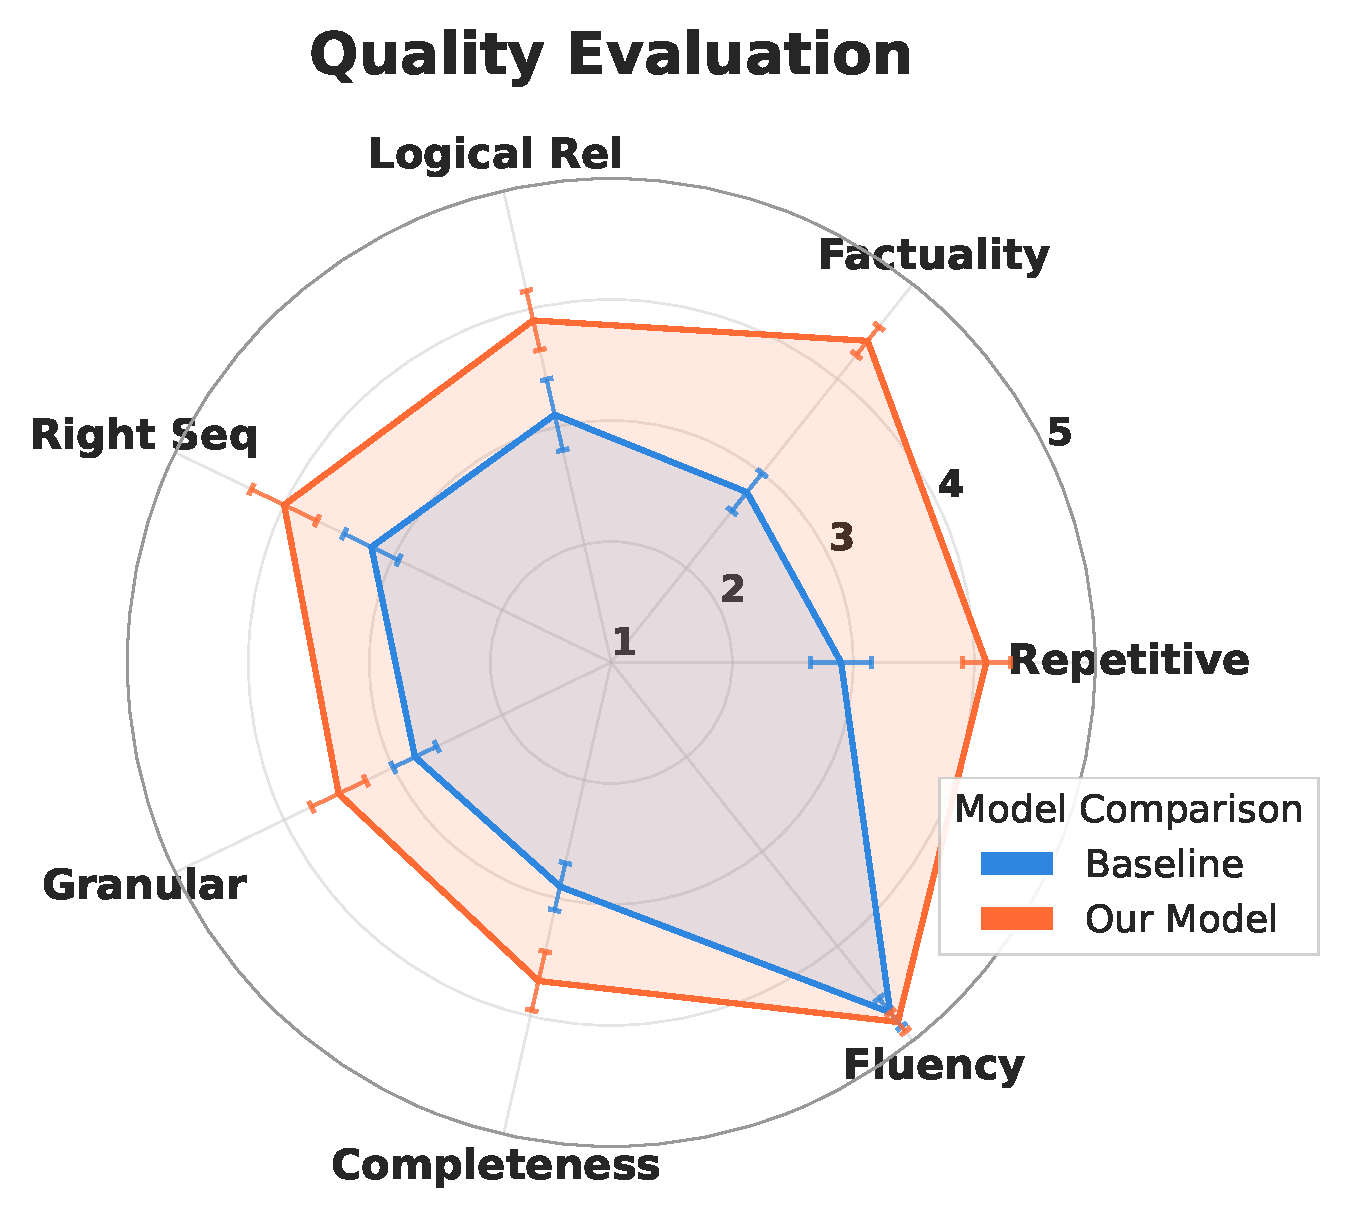
\includegraphics[width=0.65\linewidth]{01.Figures/radar_comparison_chart.pdf}
\caption{Human evaluation of generated sub-questions: Graph-CPO vs.\ the Qwen3-32B baseline, showing mean and standard deviation over 400 MWPs rated by four raters.}
\label{fig:comparison_}
\end{figure}

Figure~\ref{fig:comparison_} shows that Graph-CPO consistently outperforms the Qwen3-32B baseline on all non-fluency dimensions. The largest gains appear in factuality (4.3 vs.\ 3.5) and correct sequencing (4.4 vs.\ 3.6), indicating that graph-grounded optimization better aligns questions with the mathematical dependencies of the problem. Both methods achieve high fluency, but Graph-CPO yields more stable scores across structural criteria such as completeness, granularity, and logical relevance.

\textit{Qualitative case study.}
A worked example comparing Graph-CPO's generated question sequence with the baseline for a representative MWP is given in Appendix~\ref{app:example} (Table~\ref{tab:qual_example}).

\paragraph{Ethical considerations.}
The human study involved four mathematics researchers who voluntarily participated and consented to rate anonymized question outputs; no student or personal data were used. The generated sub-questions are intended as supplemental scaffolds rather than as answer keys, and downstream deployments should pair them with answer verification to avoid leaking solutions to learners.



\section{Conclusion}

We introduced a novel framework for generating effective Socratic sub-questions for Math Word Problems by modeling the process as a finite-horizon sequential decision task anchored to a Semantic Dependency Graph. This structural grounding reduces reasoning error rates from 24.5\% to 1.2\% and achieves a 95.6\% sequence validity rate through decoupled reward normalization and curriculum-based weighting that prevent reward collapse.
Beyond automated math tutoring, our work demonstrates that explicitly modeling task structure through dependency graphs can substantially enhance reinforcement learning for generation tasks with complex compositional requirements. The success of treating heterogeneous reward signals as independently scaled dimensions rather than scalar aggregates suggests broader applicability to multi-objective optimization in language generation. Future work should explore cross-domain generalization to other structured reasoning tasks and investigate personalization strategies that adapt question sequencing to individual learner knowledge states.
\label{sec:conclusion_end} %% TEMP page-budget gauge — remove at camera-ready

%%
%% The next two lines define the bibliography style to be used, and
%% the bibliography file.
\bibliographystyle{ACM-Reference-Format}
\bibliography{sample-base}


\section{Appendix}


\subsection{Training Hyperparameters}

\begin{table}[H]
\centering
\footnotesize
\caption{Graph-CPO training hyperparameters.}
\label{tab:hyperparams}
\begin{tabular}{ll}
\toprule
\textbf{Parameter} & \textbf{Value} \\
\midrule
\multicolumn{2}{l}{\textit{Model Architecture}} \\
Backbone & Qwen3-32B \\
Fine-tuning & LoRA $r=64$, scaling 128, attn.+MLP \\
Trainable parameters & ${\sim}190$M \\
GNN layers ($L$) & 3 \\
GNN hidden dimension & 768 \\
Graph prefix dimension & 1024 \\
\midrule
\multicolumn{2}{l}{\textit{Data}} \\
Silver-labeled SDG training problems & 12{,}000 \\
Teacher Socratic sequences (warm-start) & 8{,}000 MWPs \\
\midrule
\multicolumn{2}{l}{\textit{Supervised Warm-Start (Section 3.3)}} \\
Learning rate & 2e-5 \\
Batch size & 16 per GPU \\
Gradient accumulation & 4 steps \\
Warm-up steps & 500 \\
Epochs & 3 \\
\bottomrule
\end{tabular}
\end{table}

\begin{table}[!ht]
\centering
\footnotesize
\caption{Graph-CPO training hyperparameters (continued).}
\label{tab:hyperparams_cont}
\begin{tabular}{ll}
\toprule
\textbf{Parameter} & \textbf{Value} \\
\midrule
\multicolumn{2}{l}{\textit{Graph-CPO RL Training (Section 3.4)}} \\
Learning rate & 1e-5 \\
RL epochs & 50 \\
Rollouts per prompt ($M$) & 8 \\
KL coefficient ($\beta$) & 0.01 \\
Clip threshold ($\epsilon_c$) & 0.2 \\
Curriculum decay ($\lambda$) & 0.01 \\
$\omega_{\min}$ / $\omega_{\max}$ & 0.1 / 0.8 \\
Anchor schedule ($\alpha_0$, $\alpha_{\min}$, $\lambda_\alpha$) & 0.8, 0.05, 0.01 \\
Contrastive penalty ($\eta$) & 0.5 \\
Similarity threshold ($\tau_{\mathrm{sim}}$) & 0.75 \\
NLI threshold ($\tau_{\mathrm{nli}}$) & 0.6 \\
\midrule
\multicolumn{2}{l}{\textit{Frontier Node Selection (Eq. 2)}} \\
$\lambda_g$ / $\lambda_d$ / $\lambda_c$ / $\lambda_r$ & 0.4 / 0.3 / 0.2 / 0.1 \\
\bottomrule
\end{tabular}
\end{table}

\subsection{Computational Cost Analysis}
\label{sec:cost_app}

Table~\ref{tab:cost_analysis} reports training and inference cost. GPU-hours are computed as wall-clock time multiplied by the number of GPUs.

\begin{table}[t]
\centering
\caption{Computational cost comparison. GPU-h is total training cost on 4 A100-40GB GPUs: the SFT row is measured over 50 SFT epochs and the RL rows over 50 RL epochs; the 3-epoch warm-start initialization adds about 20 GPU-h. Lat. denotes average generation time per problem.}
\label{tab:cost_analysis}

\setlength{\tabcolsep}{3pt}
\begin{tabular}{lcccc}
\toprule
\textbf{Method} & \textbf{Time/ep.} & \textbf{GPU-h} & \textbf{Lat.} & \textbf{Mem.} \\
 &  &  & \textbf{(s)} & \textbf{(GB)} \\
\midrule
Qwen3-32B SFT & 0.17h & 34 & 2.4 & 32.1 \\
GRPO scalar & 3.05h & 610 & 5.4 & 38.7 \\
Graph-CPO & 3.18h & 636 & 5.6 & 39.1 \\
Graph-CPO w/o NLI & 2.36h & 472 & 3.8 & 37.8 \\
\bottomrule
\end{tabular}

\end{table}

Graph-CPO is more expensive than SFT because RL requires multiple rollouts and reward computation. However, its overhead over scalar GRPO is small, since dynamic reward normalization and graph-prefix conditioning add little cost. The main extra cost comes from NLI-based coherence scoring: removing NLI reduces training time from 3.18h to 2.36h per epoch and latency from 5.6s to 3.8s. Graph construction is performed offline and cached, while NLI scoring is batched across rollouts.

\subsection{Training Rewards Comparison}
\label{sec:training_curves}

\begin{figure*}[!ht]
\centering
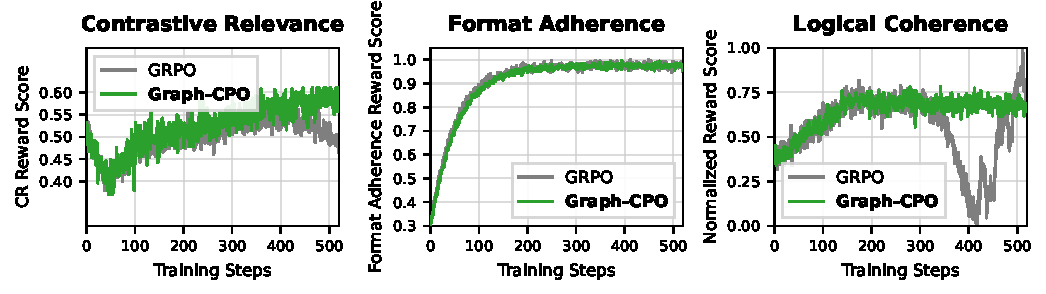
\includegraphics[width=0.80\linewidth]{01.Figures/complete_training_metrics_analysis.pdf}
\caption{Training behavior of GRPO and Graph-CPO across Contrastive Relevance, Format Adherence, and Logical Coherence rewards on Qwen3-32B.}
\label{fig:training_comparison}
\end{figure*}

From the training curves of GRPO and Graph-CPO on Qwen3-32B shown in Figure \ref{fig:training_comparison}, we observe that the Question Generator model initially tends to maximize the less complex reward dimensions regardless of the optimization framework. In this setting, the Format Adherence reward is easier to optimize, leading both GRPO and Graph-CPO to achieve near-perfect format scores within approximately the first 100 training steps. Crucially, this rapid rise in format adherence coincides with an early dip in the Contrastive Relevance reward, indicating an initial competition between the structural and semantic objectives. During this baseline phase, the model prioritizes satisfying surface-level formatting constraints, temporarily compromising the more challenging math-grounded relevance goal.


However, looking at the long-term trajectories, Graph-CPO recovers and enhances the Contrastive Relevance reward significantly more effectively than GRPO, ultimately securing higher relevance scores. This divergence becomes highly pronounced after 400 training steps, where GRPO's training begins to destabilize---evidenced by a gradual decay in its Contrastive Relevance score while Graph-CPO maintains a steady upward trajectory.
Furthermore, while both frameworks maintain near-perfect format adherence scores throughout the training horizon, we also track the logical coherence metric within each training batch to evaluate how robustly the policies preserve reasoning quality. The results show a striking contrast: as GRPO approaches the 400-step mark, its logical coherence score begins to degrade sharply, signaling a vulnerability to reward hacking where structural compliance is maintained at the expense of sound reasoning. In contrast, Graph-CPO consistently stabilizes and improves its logical coherence score, demonstrating that our graph-grounded contrastive optimization successfully prevents reward collapse.


\begin{table}[t]
\centering
\caption{Ablation of Graph-CPO reward dimensions on MathQA. DW denotes dynamic reward weighting. All variants use the same Qwen3-32B backbone and graph-conditioned action frames.}\label{tab:reward_ablation}


\setlength{\tabcolsep}{4pt}
\begin{tabular}{lccccc}
\toprule
\textbf{Variant} & $R_{\mathrm{rel}}$ & $R_{\mathrm{coh}}$ & $R_{\mathrm{form}}$ & DW & \textbf{MathQA} \\
\midrule
SFT only & -- & -- & -- & -- & 82.73 \\
GRPO scalar reward & \checkmark & \checkmark & \checkmark & -- & 84.96 \\
w/o relevance & -- & \checkmark & \checkmark & \checkmark & 78.41 \\
w/o coherence & \checkmark & -- & \checkmark & \checkmark & 83.62 \\
w/o format & \checkmark & \checkmark & -- & \checkmark & 86.18 \\
w/o dynamic weighting & \checkmark & \checkmark & \checkmark & -- & 86.47 \\
\textbf{Full Graph-CPO} & \checkmark & \checkmark & \checkmark & \checkmark & \textbf{89.60} \\
\bottomrule
\end{tabular}

\end{table}

Table~\ref{tab:reward_ablation} isolates the contribution of each reward dimension.
The SFT-only model reaches 82.73\%, showing that graph-conditioned supervised warm-starting already provides useful structural guidance, but remains below the RL-optimized variants.
Removing $R_{\mathrm{rel}}$ causes the largest degradation, dropping performance to 78.41\%, which confirms that explicit alignment with the current frontier node and penalization of resolved nodes are central to targeted Socratic questioning.
Removing $R_{\mathrm{coh}}$ also substantially reduces accuracy to 83.62\%, indicating that sequential consistency is necessary for producing useful multi-step scaffolding.
The smaller but clear drop without $R_{\mathrm{form}}$ suggests that format control mainly stabilizes parsing and optimization rather than directly encoding mathematical reasoning.
Finally, both GRPO scalar aggregation and the variant without dynamic weighting underperform full Graph-CPO, demonstrating that independently normalized rewards and curriculum-based weighting help prevent easy objectives from dominating harder pedagogical signals.




\subsection{End-to-End Example: From Problem to Socratic Questions}\label{app:example}

We illustrate the complete Graph-CPO pipeline using a representative math word problem.

\subsubsection{Input Problem}

\begin{quote}
\textit{Sarah has 24 cupcakes. She gives 8 cupcakes to her friend Tom and then bakes 15 more cupcakes. If she wants to pack all her cupcakes into boxes that hold 5 cupcakes each, how many boxes will she need?}
\end{quote}

\subsubsection{Phase 1: Graph Construction}

The pipeline extracts typed nodes and relations, producing the dependency graph below.

\begin{figure}[h]
\centering
\small
\begin{verbatim}
{v1: "Sarah has 24", v3: "gives 8 to Tom"}
        --> v5: Op(-) --> v6: after giving
{v6, v7: "bakes 15 more"}
        --> v8: Op(+) --> v9: total cupcakes
{v9, v10: "boxes hold 5"}
        --> v11: Op(div) --> v13: goal (boxes needed)
{v12: condition: ceiling (round up)}
        --> v11
\end{verbatim}
\caption{Semantic Dependency Graph of the running example expressed as prerequisite edges (prerequisite $\rightarrow$ dependent).}
\label{fig:example_dag}
\end{figure}

Key extracted nodes: $v_1$ (24 cupcakes), $v_3$ (8 given), $v_5$ (subtraction op), $v_6$ (intermediate result), $v_7$ (15 baked), $v_8$ (addition op), $v_9$ (total), $v_{10}$ (box size: 5), $v_{11}$ (division op), $v_{13}$ (goal: boxes needed).

After 3 GNN layers, each node obtains a contextual embedding incorporating its prerequisites and downstream dependencies.

\subsubsection{Phase 2: Warm-Start Initialization}

The policy $\pi_\theta$ (Qwen3-32B) is initialized via supervised learning on annotated Socratic sequences, ensuring fluent question generation before RL optimization.

\subsubsection{Phase 3: Graph-CPO Sequential Generation}

Table~\ref{tab:example_generation} shows the step-by-step generation process:

\begin{table*}[t]
\centering
\small
\caption{Graph-CPO generation trace showing frontier evolution and targeted questions.}
\label{tab:example_generation}
\begin{tabularx}{\textwidth}{cXlX}
\toprule
\textbf{Step} & \textbf{Resolved Nodes} & \textbf{Frontier} & \textbf{Generated Question} \\
\midrule
$t=0$ & $\emptyset$ & $\{v_1, v_3, v_7, v_{10}\}$ & -- \\
\midrule
$t=1$ & $\emptyset$ & $v_1$ selected & \textit{How many cupcakes does Sarah have at the start?} \\
\midrule
$t=2$ & $\{v_1\}$ & $v_3$ selected & \textit{How many cupcakes does Sarah give to Tom?} \\
\midrule
$t=3$ & $\{v_1, v_3\}$ & $v_5, v_6$ selected & \textit{After giving 8 to Tom, how many does Sarah have left?} \\
\midrule
$t=4$ & $\{v_1, v_3, v_5, v_6\}$ & $v_7, v_8, v_9$ selected & \textit{After baking 15 more, what is Sarah's new total?} \\
\midrule
$t=5$ & $\{v_1, \ldots, v_9\}$ & $v_{10}, v_{11}, v_{13}$ selected & \textit{If each box holds 5 cupcakes, how many boxes will she need?} \\
\bottomrule
\end{tabularx}
\end{table*}

\paragraph{Key mechanisms:}

\textbf{1. Frontier Tracking:} At each timestep, only nodes whose prerequisites are resolved enter the frontier. For example, $v_5$ (subtraction operation) becomes available only after both $v_1$ and $v_3$ are resolved.

\textbf{2. Contrastive Relevance:} At $t=3$, the reward computation is:

$$
R_{\text{rel}}(q_3, v_5) = \cos(\text{Enc}(q_3), \mathbf{h}_{v_5}) - 0.5 \times \max_{u \in \{v_1, v_3\}} \cos(\text{Enc}(q_3), \mathbf{h}_u)
$$

This encourages alignment with the current target ($v_5$) while penalizing repetition of resolved nodes ($v_1, v_3$).

\textbf{3. Curriculum Weighting:} Early in training ($u \approx 25$), format adherence receives weight $\omega_{\text{form}} \approx 0.65$. By $u=250$, this decays to $\omega_{\text{form}} \approx 0.16$, shifting emphasis toward relevance and coherence.

\subsubsection{Comparison with Baseline Methods}

\begin{table*}[t]
\centering
\small
\caption{Question sequences generated by different methods for the same problem.}
\label{tab:example_comparison}
\begin{tabularx}{\textwidth}{lX}
\toprule
\textbf{Method} & \textbf{Generated Questions} \\
\midrule
\textbf{Generic QG} &
1. What is this problem about? \newline
2. What operations do you see? \newline
3. Can you solve it? \\
\midrule
\textbf{Keyword-based} &
1. How many cupcakes in total? \quad \textcolor{red}{[skips intermediate steps]} \newline
2. What does Sarah do? \quad \textcolor{red}{[too vague]} \newline
3. How many boxes? \quad \textcolor{red}{[violates prerequisite order]} \\
\midrule
\textbf{Qwen3-32B baseline} &
1. How many cupcakes does Sarah start with? \newline
2. How many after baking more? \quad \textcolor{red}{[skips subtraction step]} \newline
3. How do you pack them? \\
\midrule
\textbf{Graph-CPO (ours)} &
1. How many cupcakes does Sarah have at the start? \newline
2. How many cupcakes does Sarah give to Tom? \newline
3. After giving 8 to Tom, how many does Sarah have left? \newline
4. After baking 15 more, what is Sarah's new total? \newline
5. If each box holds 5, how many boxes will she need? \\
\bottomrule
\end{tabularx}
\end{table*}

\textbf{Observations:} Generic and keyword-based methods produce questions that are either too vague or violate dependency order. The Qwen3-32B baseline generates reasonable questions but skips the subtraction step, creating a logical gap. Graph-CPO follows the exact dependency topology, generating five targeted questions that scaffold the complete reasoning path.

\paragraph{Qualitative comparison with the baseline.}
Table~\ref{tab:qual_example} provides a representative side-by-side example. The MWP is:
\textit{Maria has 12 apples. She buys 5 more apples and then gives 4 apples to her brother. How many apples does Maria have now?}
The extracted SDG path is:
$12,5 \rightarrow (+) \rightarrow$ subtotal; subtotal,$4 \rightarrow (-) \rightarrow$ goal.

\begin{table}[H]
\centering
\footnotesize
\caption{Qualitative comparison of generated Socratic sub-questions.}
\label{tab:qual_example}

\begin{tabularx}{\linewidth}{c l X X}
\toprule
\textbf{Step} & \textbf{Target node} & \textbf{Graph-CPO question} & \textbf{Baseline question} \\
\midrule
1 & Initial quantity
& How many apples does Maria have before any changes occur?
& What is the story about? \\
\addlinespace
2 & Addition / subtotal
& After Maria buys 5 more apples, what is her total before giving any away?
& Can you add the numbers? \\
\addlinespace
3 & Subtraction / goal
& After finding that subtotal, what calculation represents giving 4 apples to her brother?
& What is the final answer? \\
\bottomrule
\end{tabularx}

\end{table}

Graph-CPO follows the SDG topology by first identifying the initial quantity, then deriving the intermediate subtotal, and finally targeting the subtraction needed for the goal. In contrast, the baseline questions are more generic and less explicitly tied to the current reasoning frontier.

\subsubsection{Reward Dynamics During Training}

At training update $u=250$, for the subtraction question ($q_3$), the multi-objective advantage computation proceeds as follows:

Given 8 rollouts with mean rewards $\mu_{\text{rel}}=0.82$, $\mu_{\text{coh}}=0.88$, $\mu_{\text{form}}=1.0$ and standard deviations $\sigma_{\text{rel}}=0.07$, $\sigma_{\text{coh}}=0.05$, $\sigma_{\text{form}}=0.0$, the advantage for a rollout with rewards $(0.88, 0.91, 1.0)$ is:

\begin{align}
A_{\text{rel}} &= \frac{0.88 - 0.82}{0.07} = 0.86 \\
A_{\text{coh}} &= \frac{0.91 - 0.88}{0.05} = 0.60 \\
A_{\text{form}} &= 0.0 \quad \text{(all rollouts have perfect format)}
\end{align}

With curriculum weights $\omega_{\text{form}}(250)=0.16$ and $\omega_{\text{rel}}(250)=\omega_{\text{coh}}(250)=0.42$:

$$
\hat{A} = 0.42 \times 0.86 + 0.42 \times 0.60 + 0.16 \times 0.0 = 0.61
$$

This positive advantage increases the probability of generating similar questions. Critically, independent normalization prevents the saturated format reward from dominating the learning signal.



\section{Limitations}

While Graph-CPO demonstrates strong performance, several limitations warrant discussion. First, the Semantic Dependency Graph construction pipeline achieves 94.3\% critical path preservation but still introduces some structural errors, particularly for problems with implicit operations or complex multi-hop reasoning. Second, our approach assumes that effective pedagogical scaffolding follows the topological structure of mathematical dependencies, which may not capture all aspects of human learning, such as conceptual difficulty or metacognitive considerations. Third, computational cost remains higher than supervised baselines due to rollout sampling during RL training, though this overhead is modest compared to scalar GRPO (636 vs 610 GPU-hours). Finally, our evaluation focuses on mathematical reasoning; the generalizability to other domains requiring structured scaffolding (e.g., physics problem-solving, logical argumentation) remains to be investigated.

\end{document}
\endinput
%%
%% End of file `main.tex'.
